\documentclass[12pt]{article}

% Language setting
\usepackage[utf8]{inputenc}
\usepackage[bulgarian]{babel}

% --------------------- Packages  --------------------
% Use biblatex
\usepackage{biblatex}
\addbibresource{bibliography.bib}
% Table thickness
\usepackage{ctable}
% Equations: SI units
\usepackage{siunitx}
% Approximately equal
\usepackage{amssymb}
% degrees symbol
\usepackage{gensymb}
% warning box
\usepackage{pifont,mdframed}
% Multiline math
\usepackage{amsmath}

\newenvironment{warning}
  {\par\begin{mdframed}[linewidth=2pt, linecolor=white]%
    \begin{list}{}{\leftmargin=1cm
                   \labelwidth=\leftmargin}\item[\Large\ding{43}]}
  {\end{list}\end{mdframed}\par}

% --------------------- Title  --------------------
\addbibresource{bibliography.bib}

\begin{document}

% Anfang der Titelseite________________________________________________________________________________
\begin{titlepage}
	\flushleft
	{\scshape\Large Протокол III \hspace{2cm} Молекулна физика\par}
	\vspace{4cm}
	{\huge\bfseries Измерване на коефициента на топлопроводимост на твърди тела\par}
	\vspace{1cm}
	{\LARGE\bfseries Лабораторно упражнение №3.17\par}
	\vspace{5cm}
    {\LARGE\bfseries Виолета Кабаджова, \par}
    {\large\bfseries ККТФ, фак. номер: 3PH0600026\par}
	\vspace{1cm}
	
	{\large Физически Факултет, 
	
	Софийски Университет "Св. Климент Охридски"
	
	4 април 2023 г.\par}
	
\end{titlepage}

\section{Теоритична част}\label{sec:theoretical-part}
Топлопроводимостта е основен механизъм за пренасяне на топлина в твърди тела. При нея се осъществява пренос само на кинетична енергия от по-топлите към по-студените части на системата, докато пренос на маса липсва.

От закона на Фурие за количество топлина, което се предава от нагревател с постоянна температура $T_H$ през хомогенна топлопроводяща среда с дебелина $h$ и напречно сечение $S$ за време $dt$, при линейно изменение на температурата следва уравнение \ref{eq:fourier-thermal-conductivity}, където $k$ е коефициентът на топлопроводимост на средата, a $T$ - температурата на термодинамичната система, която получава топлина.

\begin{equation}\label{eq:fourier-thermal-conductivity}
    \delta Q = \frac{kS}{h}(T_H - T)dt
\end{equation}

Оттук, коефициентът на топлопроводимост $k$ се дефинира като количеството топлина, което преминава за единца време през единца площ, перпендикулярна на потока топлина, при изменение на температурата с един градус на единцица дължина.

Количеството топлина, което преминава за единца време, се нарича топлинен поток q и се изразява чрез формула \ref{eq:thermal-stream}.

\begin{equation}\label{eq:thermal-stream}
    q = \frac{\delta Q}{dt} = \frac{kS(T_H - T)}{h}
\end{equation}

Когато едно тяло получи количество топлина $\delta Q$, но \textit{не извършва работа и няма топлинни загуби}, то това количество топлина се влага в повишаване на температурата на това тяло от $T$ с температура $dT$. При наличие на тези условия връзката между $\delta Q$ и $dT$ се изразява чрез форлума \ref{eq:dq-dt}, където $C$ е топлинният капацитет на тялото, като следствие от първия принцип на термодинамиката. Оттам и от уравнение \ref{eq:fourier-thermal-conductivity} следват уравнения \ref{eq:dq-dt-middle} и \ref{eq:C-k}.

\begin{equation}\label{eq:dq-dt}
    \delta Q = C dT
\end{equation}

\begin{equation}\label{eq:dq-dt-middle}
    \frac{\delta Q}{dt} = q = C\left(\frac{dT}{dt}\right)
\end{equation}

\begin{equation}\label{eq:C-k}
    C\frac{dT}{dt} = k (T_H - T_2)\frac{S}{h}
\end{equation}


Уравнение 5 изразява термодинамична система, не извършваща работа, в която обаче непрекъснато се подава топлина и има топлинни загуби. Тогава е възможно достигане на стационарно състояние на системата при достигане на постоянна температура $T$, при която потокът топлина към тази система във всеки момент ще бъде равен на подока топлина, отдаден от нея. Във формула \ref{eq:C-k} $T_1$ е температурата на нагревателя, а $T_2$ - температурата на термодинамичната система.

От формула \ref{eq:C-k} може да се изрази и формулата за определяне на коефициента на топлопроводимост на средата $k$ (ур. \ref{eq:k}), където $C$ е топлинният капацитет на охладителя, $\left(\frac{dT}{dt}\right)_{T_2}$ - скоростта на изменение на температурата на охладителя при $T_2$ и $S = \frac{\pi d^2}{4}$ в следствие от експерименталната установка, която ще бъде описана по-долу.

\begin{equation}\label{eq:k}
    k = \frac{h}{S} \frac{C}{(T_1-T_2)} \left(\frac{dT}{dt}\right)_{T_2}
\end{equation}

\section{Експериментална част}

\subsection{Експериментална установка} 
На фиг. \ref{fig:setup} е представена схема на опитната постановка. Тя включва три плочи с еднакви диаметри - нагревател, образец и охладител, като към първото и последното има закачени температурни сензори. Трите пласта се фиксират един към друг чрез корекционни винтове. 

\subsection{Задача 1: Създаване на стационарно състояние на системата нагревател-образец-охладител и измерване на температурите му $T_1$ и $T_2$}

За тази цел настройваме нагревателя на $T_1 = 65 \degree C$ и изчакваме, докато образецът достигне своята максимална температура, при която вече се фиксира и която температура остава постоянна. Това се случва при $T_2 = 45.5 \degree C$.
\begin{figure}
    \centering
    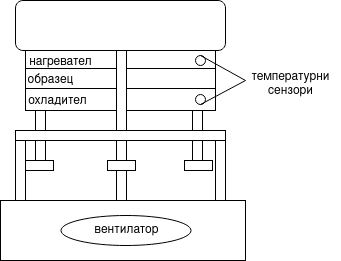
\includegraphics[width=0.5\textwidth]{images/thermal-conductivity-cooling-setup.drawio.png}
    \caption{\label{fig:setup}Схема на опитна постановка}
    \label{fig:setup}
\end{figure}

\subsection{Задача 2: Определяне на скоростта на изменение на температурата на охладителя $\left( \frac{dT}{dt}\right)_{T_2}$}
\begin{figure}
    \centering
    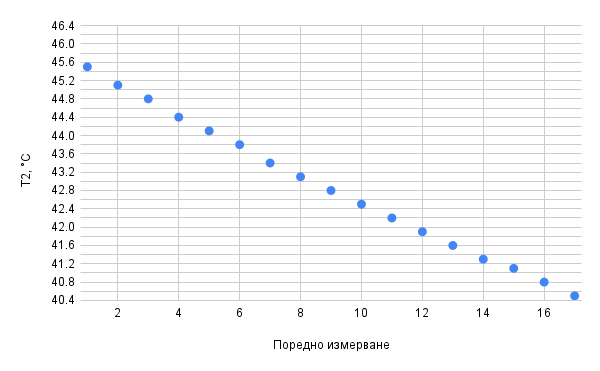
\includegraphics[width=1\textwidth]{images/chart.png}
    \caption{\label{fig:cooling-graph}Графика на охлаждане на образеца}
    \label{fig:setup}
\end{figure}

За целта отделяме нагревателя от образеца и оставяме образецът да изстине, като на всеки 10 секунди записваме стойността на температурата му. Получените стойности илюстрираме на графиката на фиг. \ref{fig:cooling-graph}. Оттук забелязваме, че графиката на охлаждане за измерения период е линейна, като разликата между всеки две стойности на поредни измервания е средно $0.31\pm0.02 \degree C = \left[\frac{dT}{dt}\right]^{*}_{T_2}$. Това съответства на стойността на охлаждането на образеца чрез отдаване на топлина от всичките му повърхнини $S^* = \frac{\pi d^2}{2} + \pi d h$, докато търсената стойност е тази на скоростта на охлаждане при излъчване само от долната основа на образеца $S = \frac{\pi d^2}{4} + \pi d h_o$. Следователно скоростта на охлаждане при излъчване от единица площ е $\frac{1}{S^*}\left[\frac{dT}{dt}\right]^{*}_{T_2}$. Оттук скоростта на охлаждане чрез излъчване само от долната му основа е $\left[\frac{dT}{dt}\right]_{T_2} = \frac{S}{S^*}\left[\frac{dT}{dt}\right]^{*}_{T_2} = 0.0156\pm 0.0001\degree C/s$.

\subsection{Задача 3: Изчисляване на коефициента на топлопровидимост на изледвания образец}
За да намерим коефициента на топлопроводимост използваме формула \ref{eq:k} и стойностите на различните параметри, записани в таблица \ref{tbl:params} и получаваме $k = 0.15 \pm 0.08\frac{W}{m\cdot K}$.

\begin{table}[h]
\begin{center}
\begin{tabular}{|l|l|l|} \hline
        височина на образеца h & 7.5 mm \\ \hline
        диаметър на образеца d & 130 mm \\ \hline
        маса на образеца m & 865 g \\ \hline
        специфичен топлинен капацитет &  \\ 
        на охладителя c при t = 25 $\degree$C & 384 $\frac{J}{kg.K}$\\ \hline
        $T_1$ (на нагревателя) & 65 $\degree$ C\\ \hline
        $T_2$ (на охладителя) & 45.5 $\degree$ C\\ \hline
\end{tabular}
\caption{\label{tbl:params}Параметри на образеца}
\end{center}
\end{table}

\end{document}
